\chapter{Analisis dan Rancangan Sistem}

\section{Analisis Sistem}

Analisis sistem terdiri dari gambaran umum sistem yang dapat dilihat pada baguan 4.1.1 dan analisis kebutuhan sistem yang dapat dilihat pada bagian 4.1.2.

\subsection{Gambaran Umum Sistem}
\begin{figure}
    \centering
    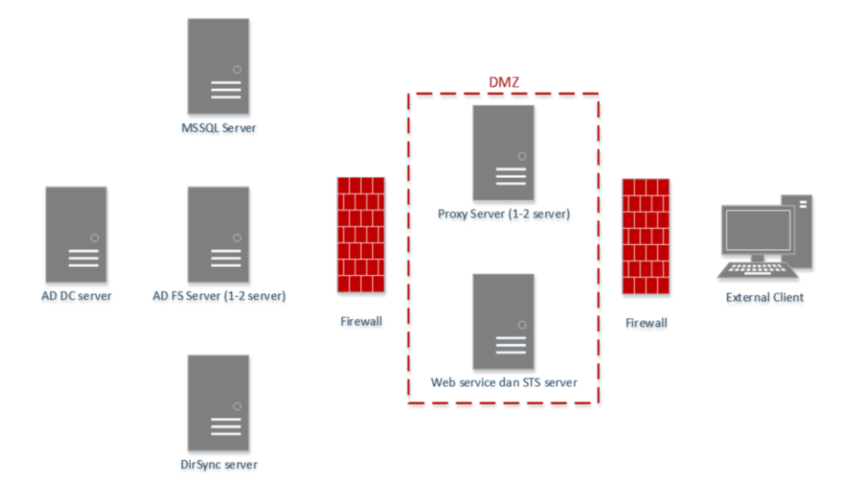
\includegraphics[width=0.8\textwidth]{contents/chapter-4/gambar-buatan-sendiri.PNG}
    \caption{Gambaran Umum Sistem}
    \label{fig:my_label}
\end{figure}
Gambar 4.2 menjelaskan secara umum system bekerja dengan menggunakan metadata login sebagai input untuk mengidentifikasi risiko dari suatu transaksi. Metadata login ini kemudian diolah dan dianalisis menggunakan metode Random Forest untuk menghasilkan prediksi risiko autentikasi dengan output nya adalah klasifikasi.

\subsection{Analisis Kebutuhan Sistem}
Dalam membangun sistem ini, diperlukan analisa kebutuhan fungsional dan non-fungsional. Kebutuhan fungsional adalah kebutuhan yang berkaitan dengan fungsi-fungsi yang harus ada dalam sistem. Kebutuhan non-fungsional adalah kebutuhan yang berkaitan dengan kualitas sistem yang dibangun. Kebutuhan fungsional dan non-fungsional dapat dilihat pada bagian 4.1 dan Tabel 4.2.

\subsubsection{Kebutuhan Fungsional}
Kebutuhan fungsional sistem ini adalah sebagai berikut:
\begin{enumerate}
    \item Sistem dapat melakukan analisis risiko autentikasi dengan menggunakan metode Random Forest.
    \item Sistem dapat men-genrate token autentikasi dari input user id.
    \item Sistem risiko autentikasi dapat terintegrasi dengan sistem FHIR.
\end{enumerate}

\subsubsection{Kebutuhan Non-Fungsional}
Kebutuhan non-fungsional sistem ini adalah sebagai berikut:
\begin{enumerate}
    \item Keamanan data : Sistem dapat melindungi data dari akses yang tidak sah.
\end{enumerate}

\section{Rancangan Sistem}
Berikut adalah rancangan sistem yang akan dibangun. Rancangan sistem terdiri dari rancangan arsitektur sistem, rancangan pembersihan data, rancangan variabel kepentingan, dan rancangan integrasi dengan sistem FHIR.

\subsection{Rancangan Arsitektur Sistem}
Rancangan arsitektur sistem dapat dilihat pada Gambar 4.3. Sistem ini terdiri dari 3 komponen utama yaitu komponen \textit{data preprocessing}, komponen \textit{data mining}, dan komponen \textit{data integration}. Komponen \textit{data preprocessing} berfungsi untuk membersihkan data dari \textit{noise} dan \textit{outlier}. Komponen \textit{data mining} berfungsi untuk melakukan analisis risiko autentikasi dengan menggunakan metode Random Forest. Komponen \textit{data integration} berfungsi untuk mengintegrasikan sistem dengan sistem FHIR.

\subsection{Rancangan Pembersihan Data}
Rancangan pembersihan data dapat dilihat pada Gambar 4.4. Pada tahap ini, data akan dibersihkan dari \textit{noise} dan \textit{outlier}. \textit{Noise} adalah data yang tidak memiliki nilai yang berarti. \textit{Outlier} adalah data yang memiliki nilai yang ekstrim. Pada tahap ini, data akan dibersihkan dari \textit{noise} dan \textit{outlier} dengan menggunakan beberapa metode yaitu :
\begin{enumerate}
    \item \textit{Outlier} : Menghapus data yang memiliki nilai yang ekstrim.
    \item \textit{Noise} : Menghapus data yang tidak memiliki nilai yang berarti.
    \item \textit{Missing Value} : Menghapus data yang memiliki nilai kosong.
\end{enumerate}
\subsection{Rancangan Variabel Kepentingan}
Rancangan variabel kepentingan akan dilakukan dengan menggunakan metode Random Forest. Metode Random Forest akan menghasilkan variabel kepentingan yang dapat dilihat pada Gambar 4.5. Variabel kepentingan ini akan digunakan untuk melakukan analisis risiko autentikasi.

\subsection{Rancangan Integrasi Dengan Sistem FHIR}
Rancangan integrasi dengan sistem FHIR dapat dilihat pada Gambar 4.6. Sistem ini akan terintegrasi dengan sistem FHIR untuk mendapatkan data login dari pasien. Data login ini kemudian akan digunakan sebagai input untuk melakukan analisis risiko autentikasi.
Untuk melakukan integrasi dengan sistem FHIR, sistem ini akan menggunakan FHIR API. FHIR API adalah sebuah API yang digunakan untuk mengakses data dari sistem FHIR. FHIR API akan mengakses data dari sistem FHIR dengan menggunakan \textit{request} dan \textit{response}.

\section{Rancangan Pengujian}
Pengujian sistem ini akan dilakukan dengan menggunakan data login dari dataset. Data login ini akan digunakan sebagai input untuk melakukan analisis risiko autentikasi. Pengujian sistem ini akan dilakukan dengan menggunakan metode \textit{10-fold cross validation}. Metode \textit{10-fold cross validation} akan membagi data menjadi 10 bagian. 9 bagian data akan digunakan sebagai data latih dan 1 bagian data akan digunakan sebagai data uji. Pengujian ini akan dilakukan sebanyak 10 kali dengan menggunakan data yang berbeda-beda. Pengujian ini akan menghasilkan nilai akurasi, presisi, \textit{recall}, dan \textit{f-measure}.